
\section{Dados}
Este é o conjunto de dados os quais trabalharemos, determinaremos coeficientes de correlação, determinação, regressão e intercepto.
	\begin{table}[H]
		\center
	\begin{tabular}{|c|c|}
		\hline
		x    & y     \\ \hline
		0.00 & 2.26  \\ \hline
		0.50 & 3.80  \\ \hline
		1.00 & 4.43  \\ \hline
		1.50 & 5.91  \\ \hline
		2.00 & 6.18  \\ \hline
		2.50 & 7.26  \\ \hline
		3.00 & 8.15  \\ \hline
		3.50 & 9.14  \\ \hline
		4.00 & 10.87 \\ \hline
		4.50 & 11.53 \\ \hline
		5.00 & 12.55 \\ \hline
	\end{tabular}
\end{table}

Após o uso do software BioEstat, que usa as fórmulas estatísticas para calcular seus resultados, chegou-se aos seguintes:

\begin{figure}[H]
	\center
	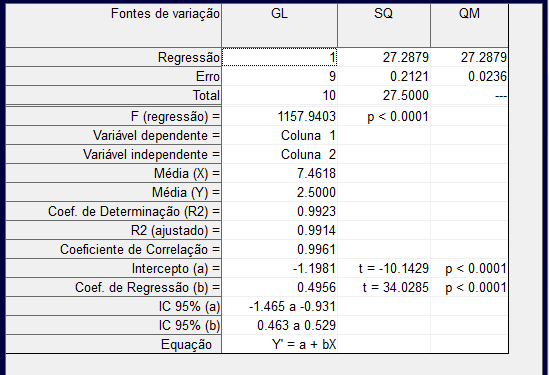
\includegraphics[scale=0.7]{imagens/reglin.png}
	\caption{Dados calculados pelo BioEstat.}
\end{figure}

\begin{figure}[H]
	\center
	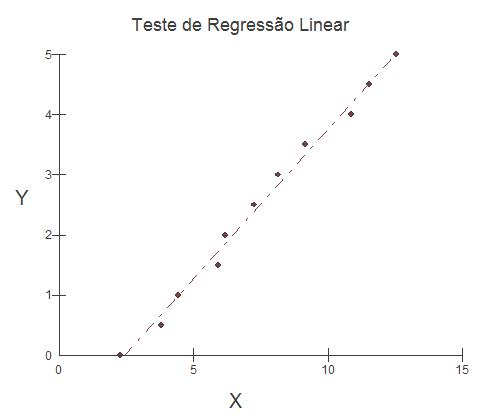
\includegraphics[scale=1]{imagens/graflin.png}
	\caption{Gráfico gerado pelo BioEstat.}
\end{figure}

Coeficiente de Regressão (Coeficiente Angular da reta): 0.4956\\
Coeficiente de Correlação: 0.9961\\
Intercepto (Coeficiente Linear): -1.1981\\
Coeficiente de Determinação: 0.9923\\


\subsection{O Programa}

O algoritmo da rede neural do Adeline será implantada através de um simples programa de computador escrito na linguagem C.


\subsection{Testando o Programa}

\begin{figure}[h]
	\center
	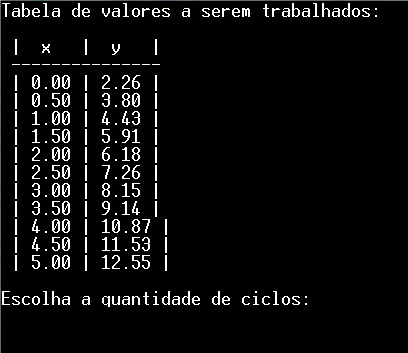
\includegraphics[scale = 1]{imagens/interf.png}
	\caption{Interface do Programa}
\end{figure}

O programa nos permite escolher a quantidade de ciclos e se os tratamento dos dados será apresentados em tempo real de execução ou se queremos apenas os resultados finais.

\begin{figure}[H]
	\center
	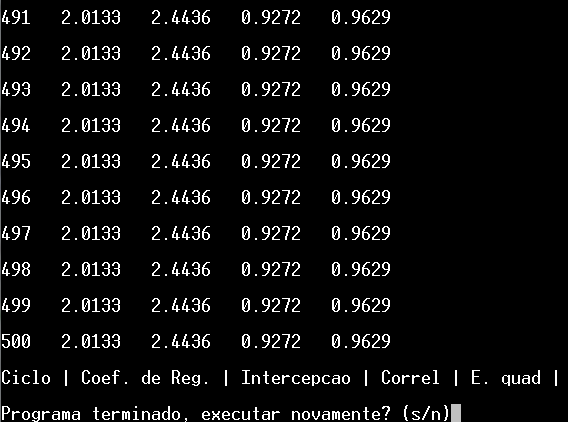
\includegraphics[scale =0.9]{imagens/real.png}
	\caption{Dados em tempo real para 500 ciclos.}
\end{figure}

\begin{figure}[H]
	\center
	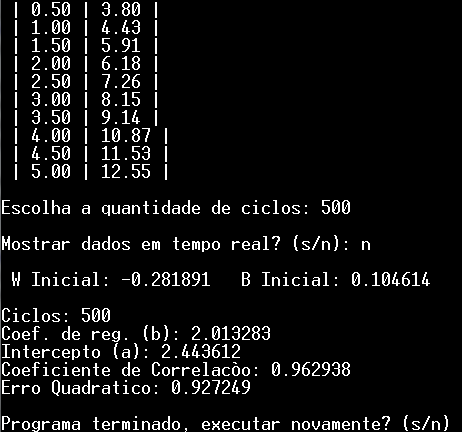
\includegraphics[scale =1]{imagens/estat.png}
	\caption{Apenas a saída final, para 500 ciclos.}
\end{figure}

Utilizando um ciclo bem alto (ordem de $10^6$), os valores permaneceram inalterados, quando comparados com 500 ciclos, o que garante que estes são os valores finais:

Coeficiente de Regressão (Coeficiente Angular da reta): 2.0133\\
Coeficiente de Correlação: 0.9272\\
Intercepto (Coeficiente Linear): 2.44636\\
Coeficiente de Determinação: 0.9629

Comparando com os dados obtidos pelo BioEstat observamos coeficientes de correlação e 
de determinação bem próximos, porém o restante divergiu por muito.
